% Autor: João Fiuza de Alencastro
% Disciplina: Segurança de Redes
% Relatório 3
\documentclass[journal]{IEEEtran}
\usepackage{listings}
\usepackage[utf8]{inputenc}
\usepackage{graphicx}




\begin{document}

\title{Relatório Frameworks}


\author{João~Fiuza~de~Alencastro~15/0131933}% <-this % stops a space




% make the title area
\maketitle


\begin{abstract}
Relatório destinado à matéria de Segurança de Redes do Departamento de engenharia Elétrica da Universidade de Brasília. Experimento realizado enfatizando a utilização de frameworks e aplicações prontas.
\end{abstract}

\begin{IEEEkeywords}
Segurança, redes, Framework, NMap, ports, TCP, UDP, vulnerabilidade.
\end{IEEEkeywords}


\IEEEpeerreviewmaketitle



\section{Introduction}
\IEEEPARstart{R}{ealizar} experimentos utilizando ferramentas específicas, melhor desenvolvidas e de fácil acesso. Frameworks oferecem a vantagem de juntar mais de uma ferramenta de descoberta de vulnerabilidades e de testes de penetração em uma só interface. Testes de penetração são realizados de forma correta quando seguem uma sequência de ações, construindo uma base de conhecimento no início e evoluindo à medida que são realizados testes, por este motivo aplicações específicas permitem ataques mais bem estruturados. \par
Serão utilizadas algumas das ferramentas já disponíveis na distribuição do Linux Kali. Essas ferramentas, são aplicações vastamente utilizadas e são um alicerce no arsenal de ataques de \textit{'hackers'} ou \textit{'ethical hackers'}. Dentre elas estão: nmap, nikto, hydra, cisco-torch e por fim, a mais completa das aplicações, o Sparta, um framework que contempla todas as ferramentas previamente citadas.

\subsection{Aplicativos}
\subsubsection{nmap}
O conhecido aplicativo nmap deve ser realizado em etapas ou fases para ser utilizado de forma correta. Isso já é um forte indicativo que a ferramenta em questão vai muito além de um simples \textit{'port scanner'}.

%Imagem
\begin{figure}[h!]
	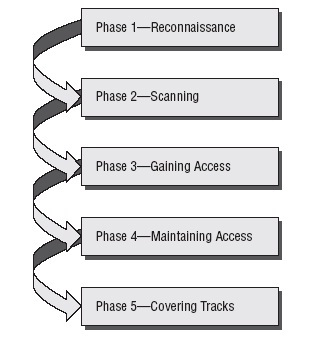
\includegraphics[width=0.65\linewidth]{../nmap_phases_pic.jpg}
	\caption{Fases de um nmap scan}
	\label{fig:nmap_phases}
\end{figure}

\subsubsection{nikto}
Baseando-se no resultado de um rápido scan no apache rodando no localhost, é visto que a ferramenta roda vários scripts de verificacão de seguranca do ambiente web. Apesar de o scan ser feito em um simples html no servidor local, o resultado é muito interessante, por mostrar o resultado de todas as verificacões. A figura abaixo mostra o resultado obtido.

%Imagem
\begin{figure}[h!]
	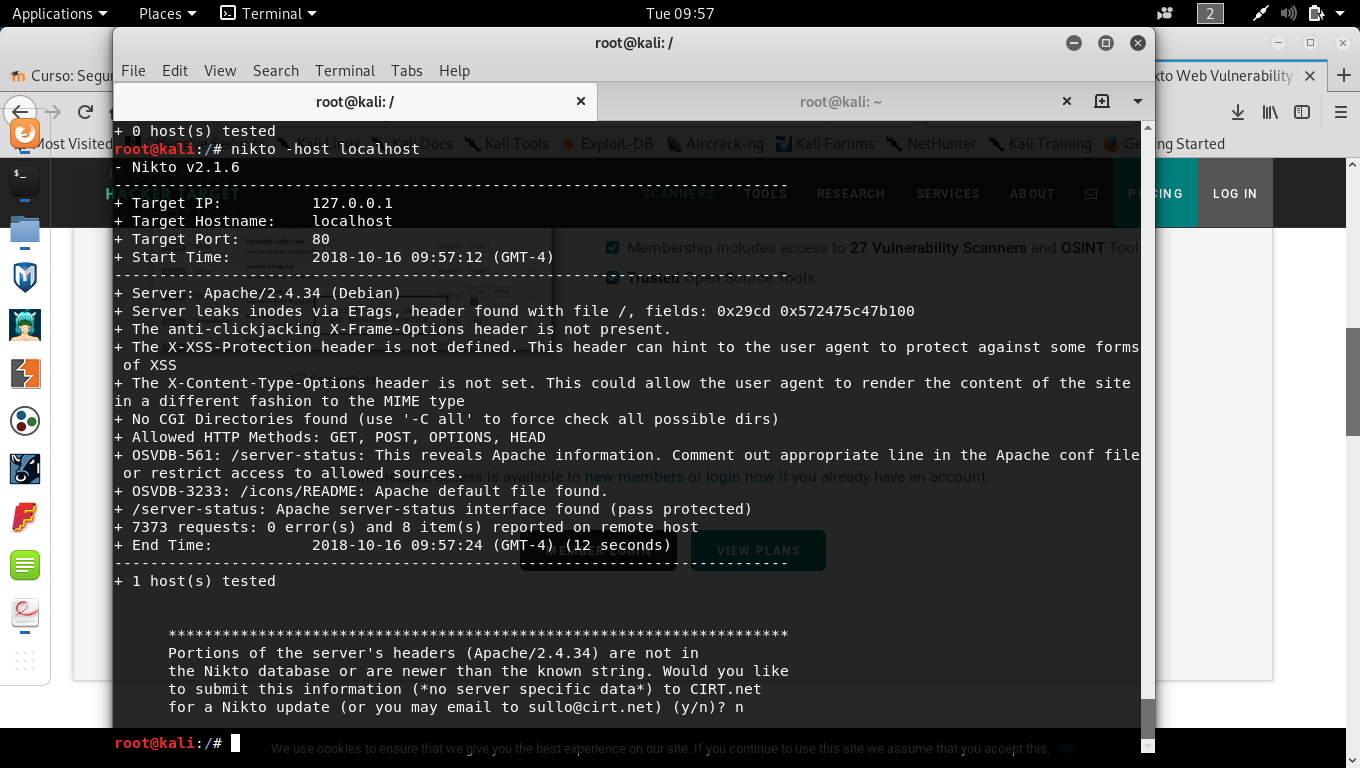
\includegraphics[width=\linewidth]{../niktoLocalhost.png}
	\caption{Resultados nikto}
	\label{fig:nikto_results}
\end{figure}

\subsubsection{hydra}
Com um resultado bem sucedido de um brute force, foi possível "quebrar" a senha de um banco de dados postgreSQL - bastante utilizado em diversas aplicações - utilizando a ferramenta Hydra. No exemplo, foi passado como parâmetro só um login, "postgres", uma lista de possíveis senhas e um host vítima do ataque. A própria ferramenta já sabe a porta padrão utilizada pelo postgreSQL, e caso a porta não fosse a padrão, a fase de pesquisa e information gathering é útil para este tipo de situação.


%Imagem
\begin{figure}[h!]
	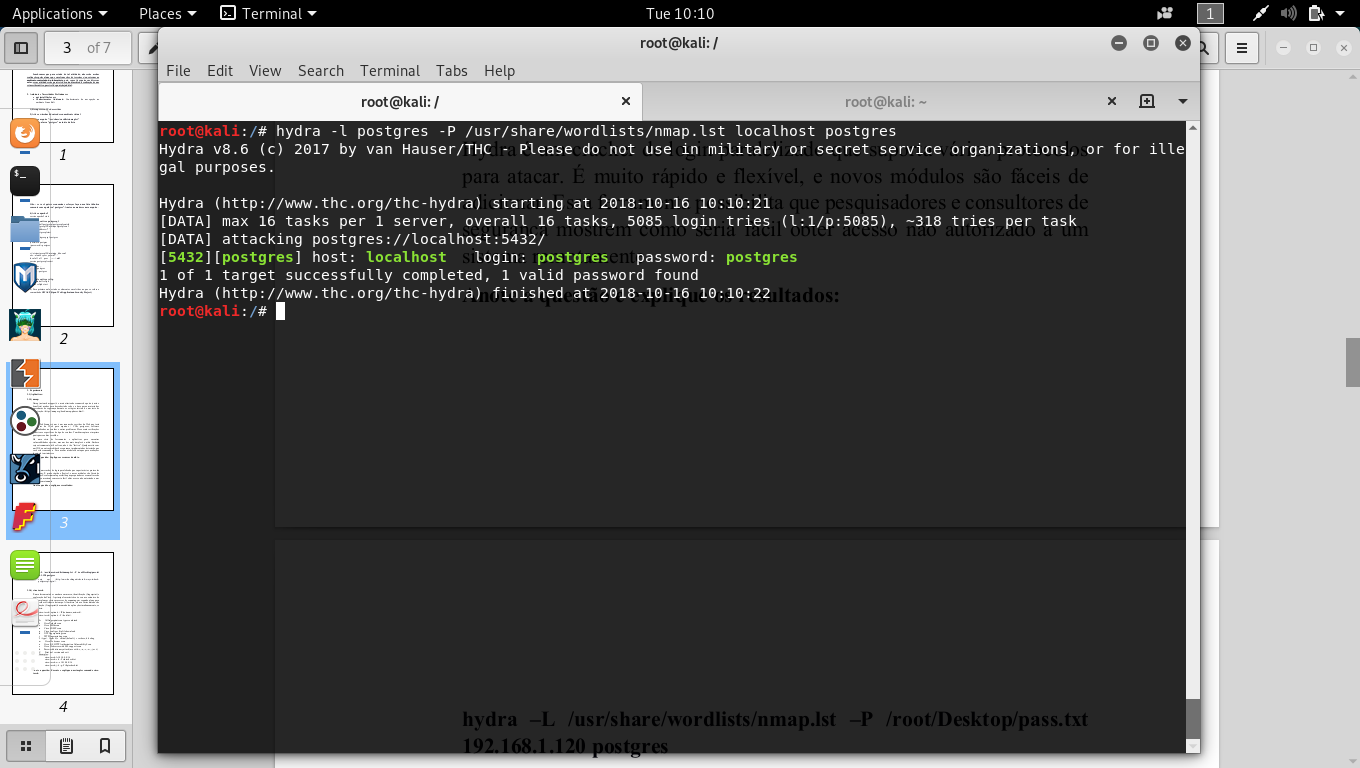
\includegraphics[width=\linewidth]{../hydraPostgresLocalhost.png}
	\caption{Resultados hydra}
	\label{fig:hydra_results}
\end{figure}

\subsubsection{cisco-torch}
Este aplicativo também é um analisador de vulnerabilidades, porém ele difere em seus métodos de análise, além de que ele distribui o processamento computacional, agilizando os procedimentos. Além disso, ele utiliza vários métodos de \textit{fingerprinting} em camada de aplicação simultaneamente. Abaixo é mostrado resultados obtidos no próprio hospedeiro local.

%Imagem
\begin{figure}[h!]
	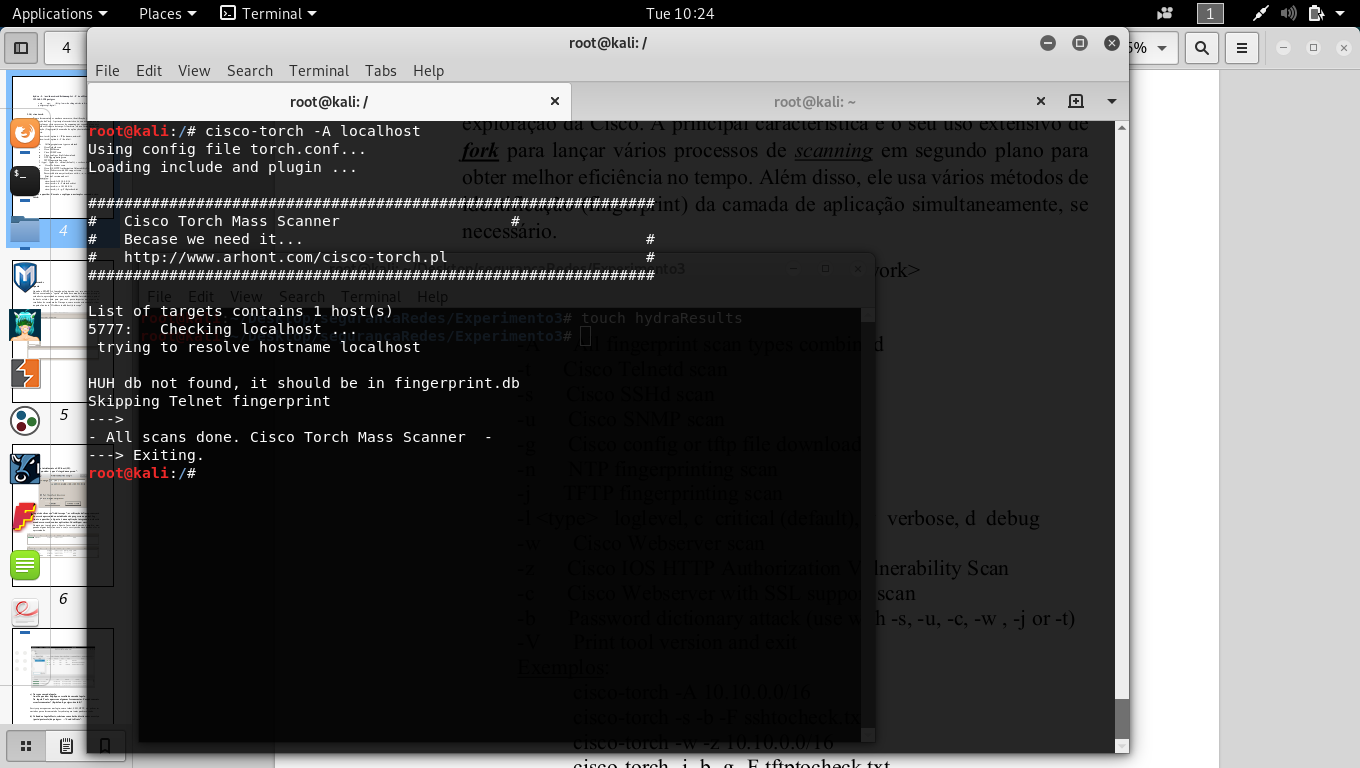
\includegraphics[width=\linewidth]{../simpleCiscoTorchLocalhost.png}
	\caption{Resultados cisco-torch}
	\label{fig:cisco_torch_results}
\end{figure}

\subsection{Frameworks}
\subsubsection{Sparta}

\section{Conclusion}



\begin{thebibliography}{1}

\bibitem{cisco-torch}
https://tools.kali.org/information-gathering/cisco-torch
\bibitem{nmap-phases}
https://nmap.org/book/nmap-phases.html
\bibitem{nmap-phases-pic}
http://amaliciousmind.blogspot.com/2013/08/nmap-step-by-step.html


\end{thebibliography}



\end{document}


